\documentclass{scrartcl}
\usepackage[utf8]{inputenc}
\usepackage{graphicx}
\usepackage{subcaption}
\usepackage{listings}
\usepackage{color}

\definecolor{dkgreen}{rgb}{0,0.6,0}
\definecolor{gray}{rgb}{0.5,0.5,0.5}
\definecolor{mauve}{rgb}{0.58,0,0.82}

\lstset{frame=tb,
  language=Java,
  aboveskip=3mm,
  belowskip=3mm,
  showstringspaces=false,
  columns=flexible,
  basicstyle={\small\ttfamily},
  numbers=none,
  numberstyle=\tiny\color{gray},
  keywordstyle=\color{blue},
  commentstyle=\color{dkgreen},
  stringstyle=\color{mauve},
  breaklines=true,
  breakatwhitespace=true,
  tabsize=3
}



\graphicspath{ {image/} }

\title{CMPE 434 - Introduction to Robotics}
\subtitle{Lab 2: Moving to Python}
\date{Deadline: September 23, 2019}

\begin{document}
\maketitle

The aim of this lab is to:
\begin{enumerate}
    \item Get acquainted with the infrastructure that will run on your EV3 bricks,
    \item Set up the programming environment on your computers,
    \item Test out our first programs on EV3 hardware.
\end{enumerate} 

\textit{EV3 Robotics Kit} comes with a brick which essentially is a small computer. Just like Windows on your PCs or iOS on your iPhones, we need to run an operating system (OS) on this computer. \textbf{ev3dev} is the name of the OS that we are going to use for this purpose. It is a \textit{Linux-based} operating system that is specifically modified to handle EV3 hardware.
\\

\begin{figure}[h!]
    \begin{center}
        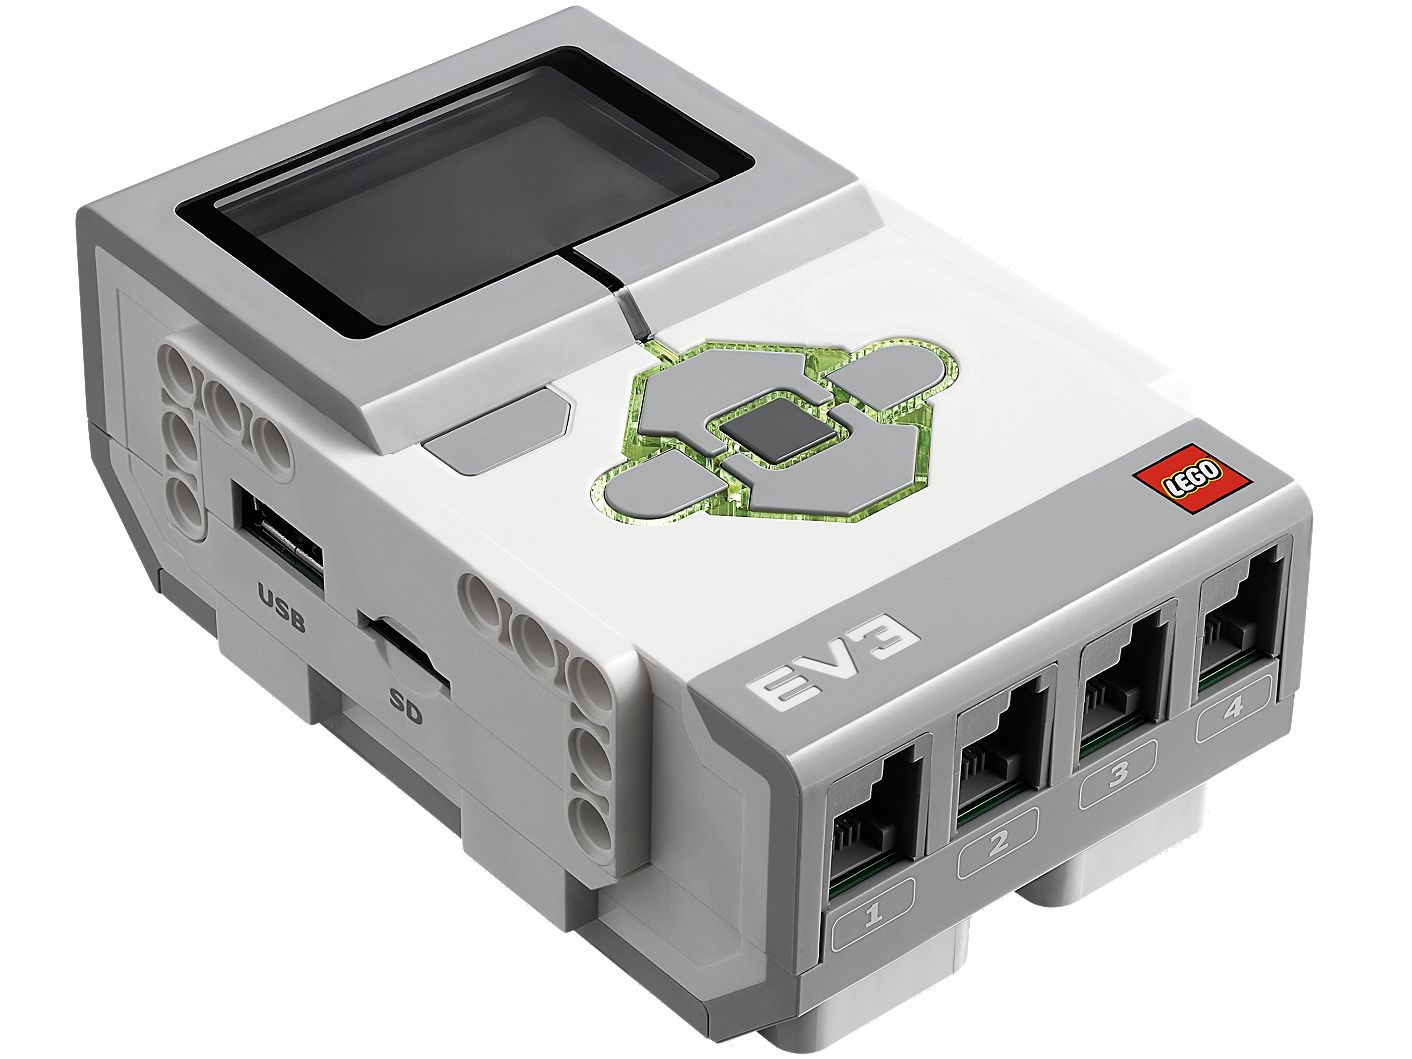
\includegraphics[width=0.5\textwidth]{brick.jpg}
        \caption{EV3 Brick}
    \end{center}
\end{figure}

By following the list below, you are expected to install \textit{ev3dev} to an SD Card and boot your brick via this medium. Then, you are asked to set up the programming environment and implement your first programs as explained below.

\newpage
\section{Things to do:}
\subsection{Setup}

\begin{enumerate}
    \item Follow the instructions at this page:\\ https://www.ev3dev.org/docs/getting-started/
    \begin{itemize}
        \item Download ev3dev-stretch image
        \item If you don't have one, download and install an image-burner to write the image into the sd card. Etcher is a free tool that you can use for this purpose https://etcher.io/
        \item Burn the image of the OS to your sd card.
        \item Boot ev3dev to see the result. In the figure below, a screenshot of a successful installation is given:
            \begin{figure}[h!]
                \begin{center}
                  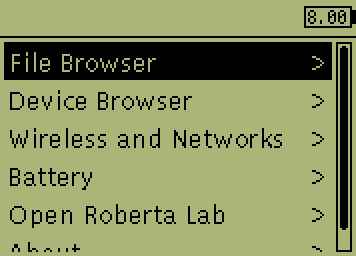
\includegraphics[width=0.3\textwidth]{main-menu.png}
                  \caption{ev3dev Main menu}
                \end{center}
            \end{figure}
    \end{itemize}
    \item Install the latest version of Python: https://www.python.org/downloads/
    \item To implement Python programs and run them on the brick, download and install Visual Studio Code (VS Code): https://code.visualstudio.com/
    \item Create your workspace, a folder to be used as the container of all your programs. Under that folder, create another one, name it \textit{lab2}.
    \item Open VS Code, and until \textit{Code completion} part, follow the \textit{Step-by-Step} guide in this address: https://github.com/ev3dev/vscode-hello-python\#step-by-step
    \item For code completion, run the following command on a command prompt: \textit{pip install python-ev3dev python-ev3dev2}

\end{enumerate}
\subsection{Fresh Project}
Now, let us create a fresh project from scratch to have further experience with ev3dev.

\begin{enumerate}
    \item Open a new window on VS Code. Under \textit{Start} click on \textit{Open folder...} directive as shown in Figure \ref{fig:fol}.
        \begin{figure}[h!]
            \begin{center}
              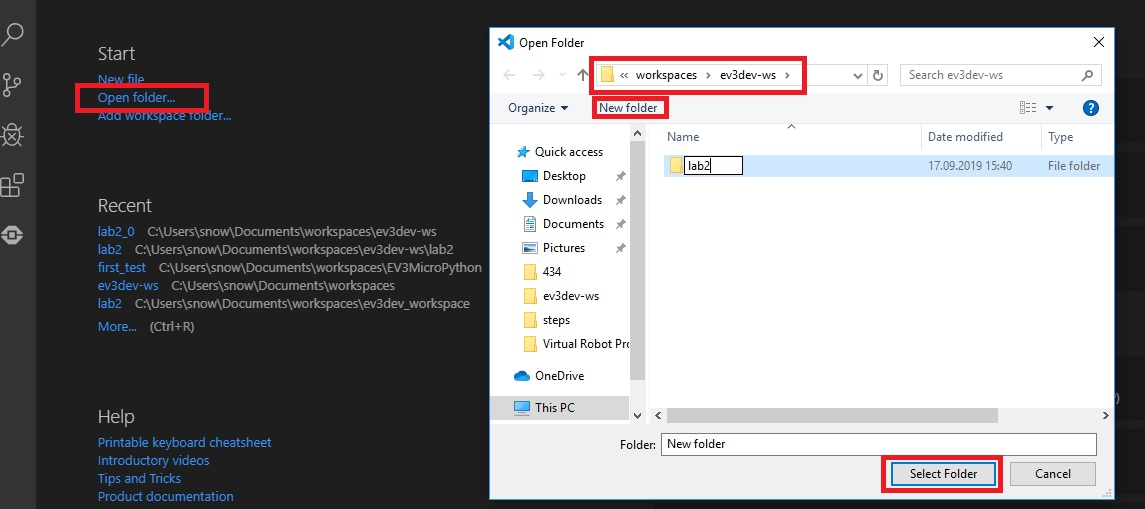
\includegraphics[width=0.75\textwidth]{fol.jpg}
              \caption{New folder}
              \label{fig:fol}
            \end{center}
        \end{figure}
    \item Create a file in this folder and name it \textit{first\_test.py}
        \begin{figure}[h!]
            \begin{center}
              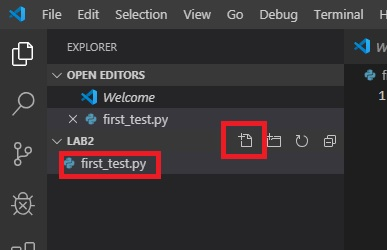
\includegraphics[width=0.35\textwidth]{ft.jpg}
              \caption{New Python file}
              \label{fig:ft}
            \end{center}
        \end{figure}
        
    \item Copy and paste the following code:
        \begin{lstlisting}
            #!/usr/bin/env python3

            from ev3dev.ev3 import *
            from time import sleep
            
            Sound.speak('Hello, I am E V 3!').wait()
            lcd = Screen()
            i=0
            
            while i<20:
                lcd.clear()
                lcd.draw.text((20+i, 20+i), 'CMPE 434')
                lcd.update()
                sleep(0.05)
                i+=1
        \end{lstlisting}

    \item Check if you can successfully connect to device form VS Code.
        \begin{itemize}
            \item Connect via USB.
            \item Make sure that the brick is already started.
            \item On \textit{EV3 Device Browser} menu, connect to the brick as shown in Figure \ref{fig:con}.
                \begin{figure}
                    \centering
                    \begin{subfigure}{.5\textwidth}
                      \centering
                      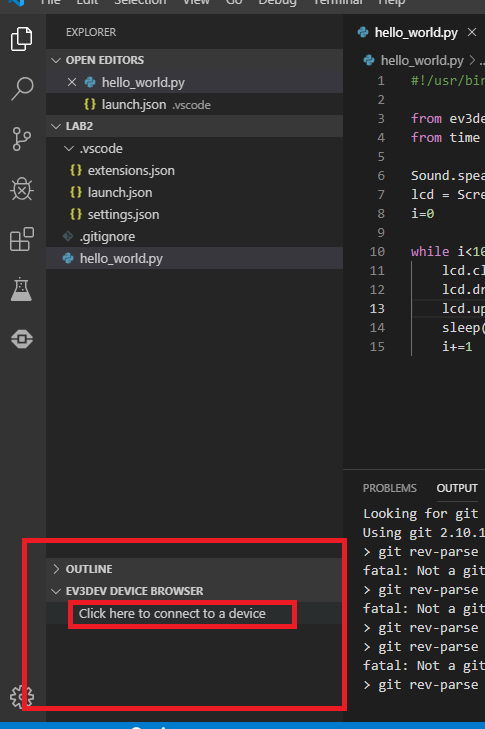
\includegraphics[width=.5\linewidth]{1.jpg}
                    \end{subfigure}%
                    \begin{subfigure}{.5\textwidth}
                      \centering
                      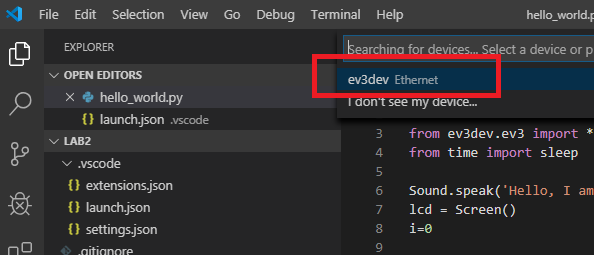
\includegraphics[width=.85\linewidth]{2.jpg}
                    \end{subfigure}
                    \caption{Connecting to the device}
                    \label{fig:con}
                \end{figure}
        \end{itemize}

    \item To run your code on the device, VS Code needs to be notified about the procedure. This process is as follows:
    \begin{itemize}
        \item Click on the \textit{Debug} button on the left-menu. Add a launch file.
            \begin{figure}[h!]
                \begin{center}
                  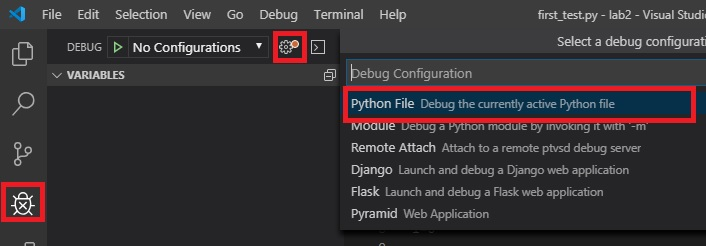
\includegraphics[width=0.75\textwidth]{r1.jpg}
                  \caption{New launch configuration}
                  \label{fig:nlc}
                \end{center}
            \end{figure}
        \item Add \textit{ev3dev} configuration as in Figure \ref{fig:ev3c}. Update it with the name of your python script and you can remove the unnecessary Python configuration as in Figure \ref{fig:unp}.
            \begin{figure}
                \centering
                \begin{subfigure}{.5\textwidth}
                  \centering
                  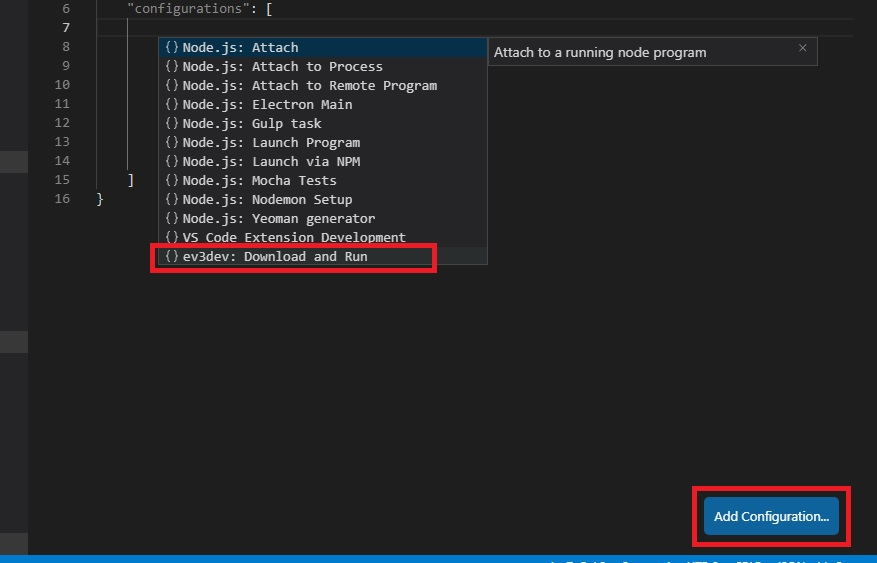
\includegraphics[width=.75\linewidth]{r2.jpg}
                  \caption{Adding ev3dev to the launch script}
                  \label{fig:ev3c}
                \end{subfigure}%
                \begin{subfigure}{.5\textwidth}
                  \centering
                  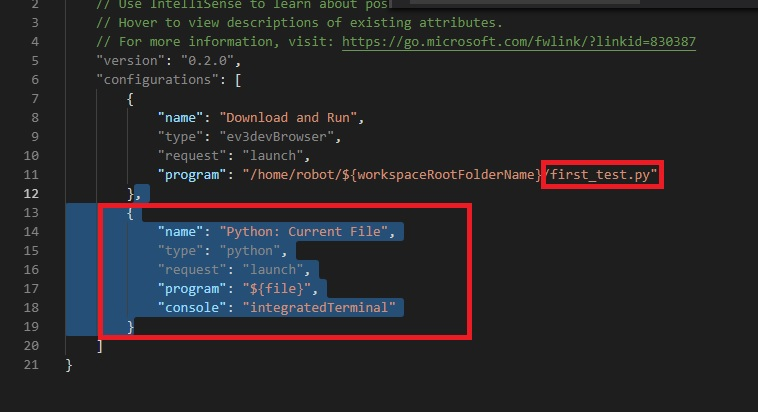
\includegraphics[width=.85\linewidth]{r3.jpg}
                  \caption{Updating the launch script}
                  \label{fig:unp}
                \end{subfigure}
                \caption{Launch script configurations}
            \end{figure}
    
        \item If everything is fine, you should be able to run your program as ın Figure \ref{fig:run}:
        \begin{figure}[h!]
            \begin{center}
              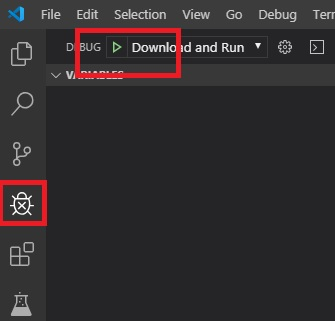
\includegraphics[width=0.5\textwidth]{run.jpg}
              \caption{Running the program}
              \label{fig:run}
            \end{center}
        \end{figure}
    \end{itemize}

\end{enumerate}

\subsection{Experiments and Requirements}
\subsubsection{Experiments:}
Now, let us experiment with other hardware parts. You may also check this page: \\https://sites.google.com/site/ev3devpython/learn\_ev3\_python/using-sensors

\underline{Ultrasonic Sensor}
    \begin{lstlisting}
        #!/usr/bin/env python3
        
        from ev3dev2.sensor.lego import UltrasonicSensor
        from ev3dev2.button import Button
        from time import sleep
        
        us = UltrasonicSensor()
        btn = Button()
        
        while(not btn.any()):
            print(us.distance_centimeters)
            sleep(0.05)
    \end{lstlisting}

\underline{Touch Sensor}
    \begin{lstlisting}
        #!/usr/bin/env python3

        from ev3dev2.sensor.lego import TouchSensor
        from time import sleep
        
        '''
        Connect both touch sensors; 1 thorugh port 1 and one through port 3
        '''
        
        ts0 = TouchSensor('in1')
        ts1 = TouchSensor('in3')
        
        while(True):
            if not ts0.is_pressed and not ts1.is_pressed:
                print('Both unpressed')
            elif ts0.is_pressed and not ts1.is_pressed:
                print('TS from port 1 is pressed')
            elif ts1.is_pressed and not ts0.is_pressed:
                print('TS from port 3 is pressed')
            else:
                break
            sleep(0.05)
    \end{lstlisting}
    
\underline{Color Sensor}
    \begin{lstlisting}
        #!/usr/bin/env python3

        from ev3dev2.sensor.lego import ColorSensor
        from ev3dev2.button import Button
        from time import sleep
        
        cs = ColorSensor()
        btn = Button()
        
        while(not btn.any()):
            print(cs.value())
            sleep(0.05)
    \end{lstlisting}
    
\underline{Gyro Sensor}
    \begin{lstlisting}
        #!/usr/bin/env python3

        from ev3dev2.sensor.lego import GyroSensor
        from ev3dev2.button import Button
        from time import sleep
        
        gs = GyroSensor()
        btn = Button()
        
        while(not btn.any()):
            print(gs.value())
            sleep(0.05)
    \end{lstlisting}
    
\underline{Motor}
    \begin{lstlisting}
        #!/usr/bin/env python3

        from ev3dev2.motor import LargeMotor, OUTPUT_A
        from time import sleep
        
        m = LargeMotor(OUTPUT_A)
        m.on(50)
        sleep(10)
        m.off()
    \end{lstlisting}

\subsubsection{Requirements:}
 Implement the \textit{Line Follower Robot} using the light sensor.
 \newpage
 
 % LINE GOES HERE
\end{document}
